\chapter{Um olhar sobre a evolução humana}\label{ch:g12:human-evolution}

Numa camada de cinza vulcânica de três milhões e meio de anos, dois
rastros de pegadas correm lado a lado por vinte e sete metros. Foram
deixados por criaturas que andavam eretas, com o calcanhar primeiro,
com o pé arqueado e o dedão alinhado com os outros --- pés como os
nossos --- numa época em que não existia cérebro maior que o de um
primata antropoide. O andar ereto veio primeiro, com dois milhões de
anos de vantagem; o cérebro, as ferramentas e a fala vieram depois, e
não em linha reta, mas ao longo de um arbusto de \omterm{def:g10:biodiversity-scales:species}{espécies}, a maioria
das quais não deixou descendentes. Este capítulo aplica as ferramentas
dos dois últimos --- caracteres compartilhados, árvores, datas, \omterm{def:g10:universal-dna:information}{DNA} ---
à linhagem que leva a nós.

\section{Os seres humanos entre os primatas}

\begin{proposition}[O nosso lugar na árvore]\label{prop:g12:human-evolution:place}
Os seres humanos são primatas: mamíferos com mãos preênseis, unhas em
vez de garras, olhos voltados para a frente e um cérebro grande para o
tamanho deles. Dentro dos primatas, os grandes primatas antropoides ---
orangotango, gorila, chimpanzé, bonobo, ser humano --- formam um \omterm{prop:g12:phylogenetic-trees:rules}{clado},
e dentro dele o chimpanzé e o bonobo são o grupo-irmão dos seres
humanos: o nosso \omterm{def:g10:universal-dna:information}{DNA} difere do deles em cerca de 1.2\% das posições, e
o ancestral comum das duas linhagens viveu uns seis a sete milhões de
anos atrás, na África. Esse ancestral não era nem um chimpanzé nem um
ser humano; as duas linhagens evoluíram desde então.
\end{proposition}
\begin{proof}[Evidence]
As matrizes de caracteres e as comparações de \omterm{def:g10:universal-dna:information}{DNA} do
\cref{ch:g12:phylogenetic-trees}: todo \omterm{def:g10:universal-dna:gene}{gene} sequenciado coloca o
chimpanzé mais perto do ser humano que do gorila, e o \omterm{def:g11:cell-cycle-mitosis:chromosome}{cromossomo} 2
humano é a fusão, ponta a ponta, de dois \omterm{def:g10:universal-dna:information}{cromossomos} que continuam
separados no chimpanzé --- e é por isso que temos 23 pares e eles 24. O
relógio molecular, calibrado nas datas fósseis de separações de
primatas mais antigas, dá a data do nó ser humano--chimpanzé.
\end{proof}

\begin{definition}[A linhagem humana]\label{def:g12:human-evolution:lineage}
A \emph{linhagem humana}\index{linhagem humana} é o \omterm{prop:g12:phylogenetic-trees:rules}{clado} de todas as
\omterm{def:g10:biodiversity-scales:species}{espécies} mais próximas dos seres humanos modernos que do chimpanzé:
tudo o que descende do lado humano do nó de seis milhões de anos. Ela
contém uma \omterm{def:g10:biodiversity-scales:species}{espécie} viva, \emph{Homo sapiens}, e umas vinte fósseis ---
os australopitecos e as várias \omterm{def:g10:biodiversity-scales:species}{espécies} do gênero \emph{Homo}. Um
fóssil pertence a ela se mostrar caracteres derivados da linhagem:
andar ereto, uma face encurtada, caninos pequenos e, mais tarde, um
cérebro grande e ferramentas.
\end{definition}

\section{Os caracteres da linhagem}

\begin{proposition}[A bipedia veio primeiro]\label{prop:g12:human-evolution:bipedalism}
O caráter derivado mais antigo da \omterm{def:g12:human-evolution:lineage}{linhagem humana} é o andar habitual
sobre duas pernas. Ele aparece no esqueleto: a abertura da base do
crânio por onde passa a medula espinal fica embaixo do crânio, e não
atrás dele, de modo que a cabeça se equilibra sobre uma coluna
vertical; a coluna tem uma curva dupla; a bacia é curta e em forma de
tigela; os fêmures se inclinam para dentro até o joelho, trazendo os
pés para baixo do centro do corpo; o pé tem um arco e um dedão alinhado
com os outros, feito para impulsionar, e não para agarrar. Tudo isso
está presente, com alguns traços de antropoide, em fósseis de quatro
milhões de anos com cérebros não maiores que o de um chimpanzé.
\end{proposition}
\begin{proof}[Evidence]
Os rastros de pegadas na cinza vulcânica, de 3.6 milhões de anos,
mostram uma passada larga com choque de calcanhar e um pé arqueado. O
esqueleto de uma australopiteca de 3.2 milhões de anos, 40\% completo,
tem bacia e joelho parecidos com os humanos e um cérebro de cerca de
\qty{400}{cm^3}. Bases de crânio da mesma idade têm a abertura medular
adiantada, embaixo do crânio. Os caracteres aparecem nesta ordem: o
andar e, depois, mais de um milhão de anos mais tarde, o crescimento do cérebro.
\end{proof}

\begin{omfigure}
\begin{tikzpicture}
  \node[anchor=south west, inner sep=0] (img) at (0,0)
    {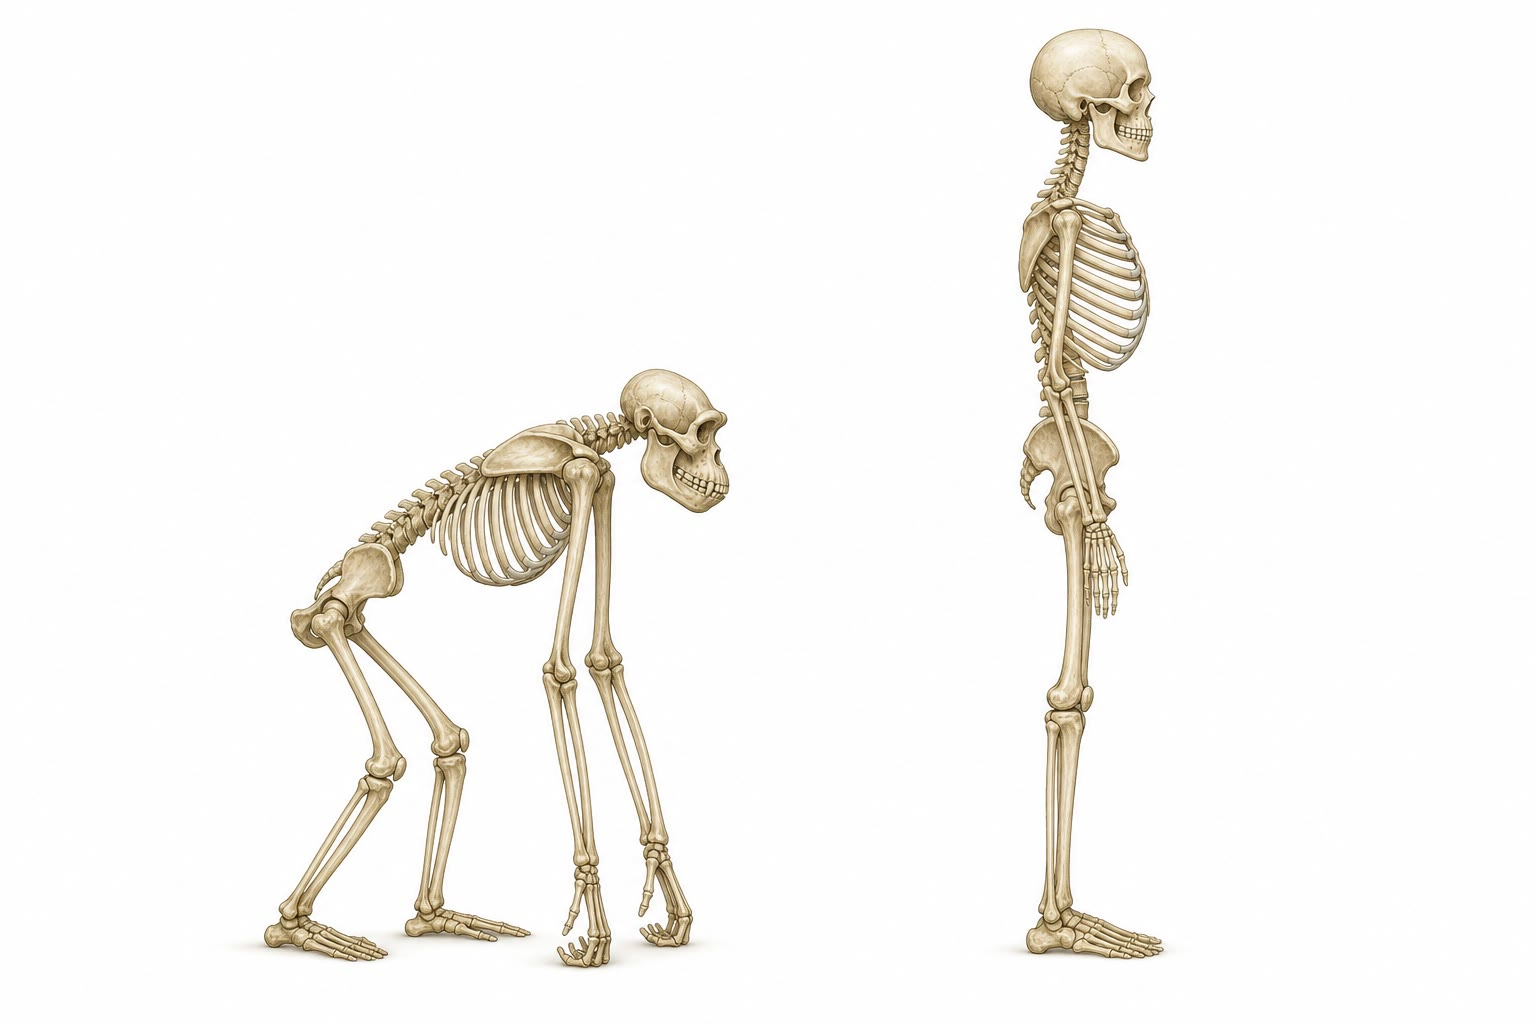
\includegraphics[width=0.56\linewidth]{images/book2/ai/fig-posture-skeletons.jpg}};
  \begin{scope}[x={(img.south east)}, y={(img.north west)},
      every node/.style={font=\scriptsize}]
    \draw[omDef, thick] (0.42,0.585) -- (0.42,0.98) node[above, align=center] {chimpanzé: abertura medular\\ na parte de trás do crânio};
    \draw[omDef, thick] (0.29,0.50) -- (-0.03,0.62) node[left, align=right] {coluna oblíqua,\\ cabeça pende\\ para a frente};
    \draw[omDef, thick] (0.23,0.42) -- (-0.03,0.40) node[left, align=right] {bacia longa\\ e estreita};
    \draw[omDef, thick] (0.25,0.26) -- (-0.03,0.18) node[left, align=right] {quadris e joelhos\\ dobrados};
    \draw[omDef, thick] (0.70,0.86) -- (1.03,0.90) node[right, align=left] {ser humano:\\ abertura medular\\ embaixo do crânio};
    \draw[omDef, thick] (0.68,0.71) -- (1.03,0.68) node[right, align=left] {coluna vertical\\ com curva dupla};
    \draw[omDef, thick] (0.70,0.54) -- (1.03,0.48) node[right, align=left] {bacia curta em\\ forma de tigela};
    \draw[omDef, thick] (0.69,0.32) -- (1.03,0.26) node[right] {joelhos sob o tronco};
  \end{scope}
\end{tikzpicture}

{\small Um esqueleto de chimpanzé e um de ser humano vistos de lado. No
antropoide, a medula espinal sai do crânio por trás e a cabeça pende
para a frente a partir de uma coluna oblíqua, sobre quadris e joelhos
dobrados; no bípede, a abertura fica embaixo do crânio, a cabeça se
equilibra sobre uma coluna vertical de curva dupla, a bacia é curta e
em forma de tigela e os joelhos ficam sob o tronco. Uma base de crânio,
uma bacia ou um joelho fósseis podem ser lidos quanto ao andar.}
\end{omfigure}

\begin{omfigure}
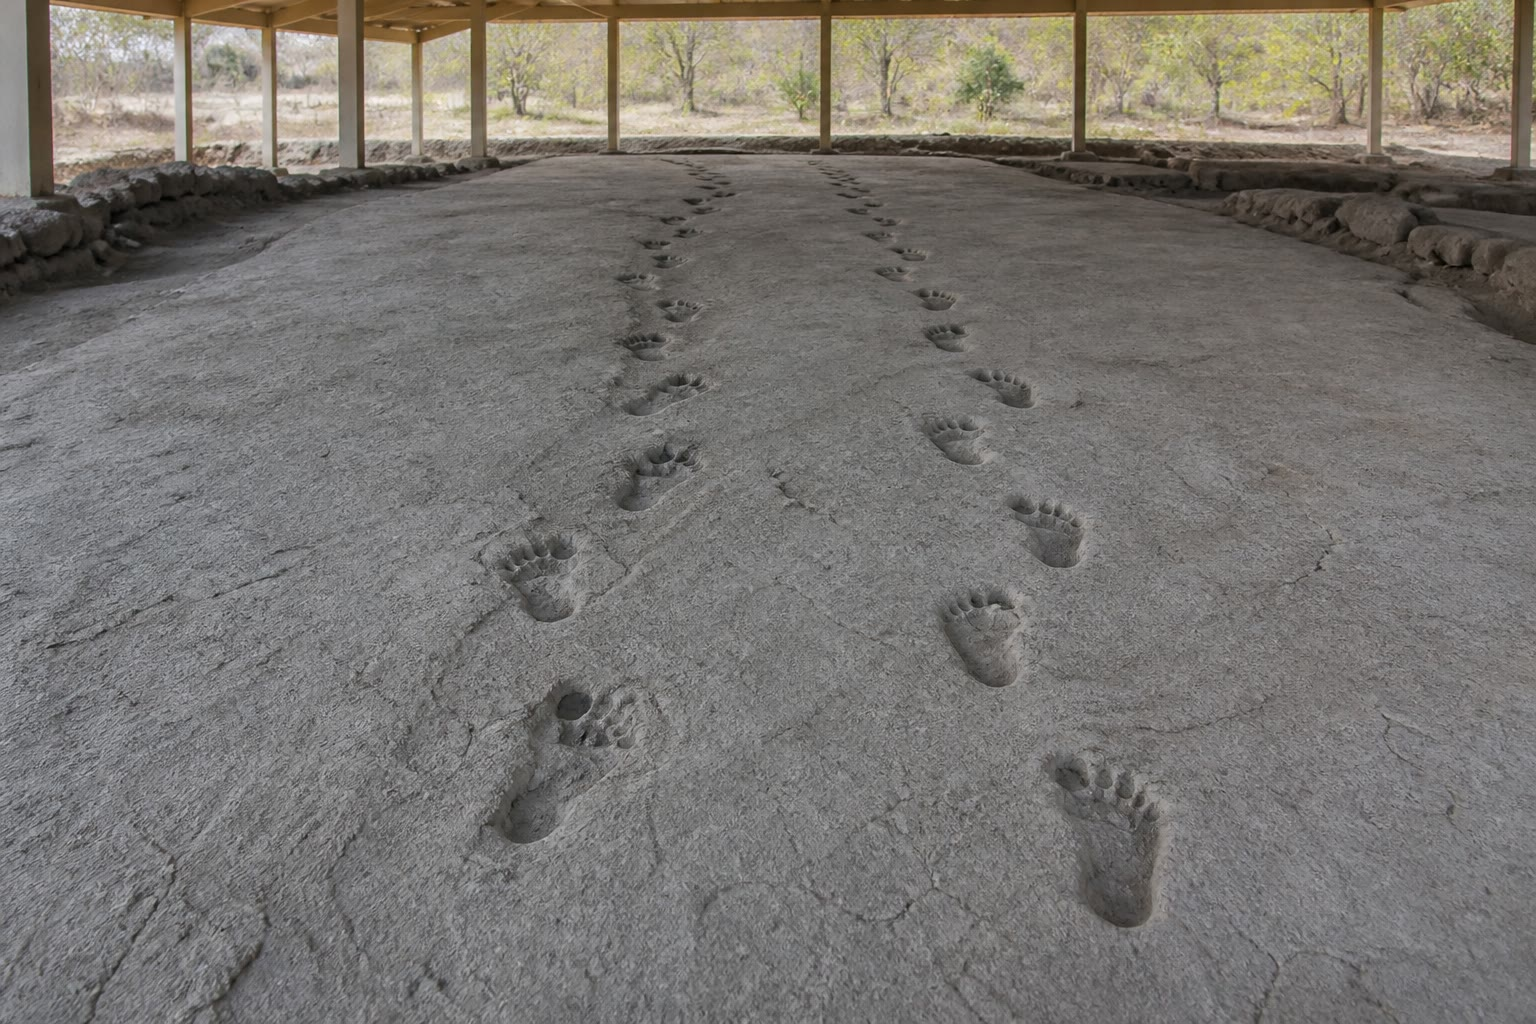
\includegraphics[width=0.6\linewidth]{images/book2/ai/g12-human-footprints.jpg}

{\small Um rastro de pegadas preservado em cinza vulcânica endurecida.
O calcanhar primeiro, um pé arqueado, o dedão alinhado: a marca de um
andarilho ereto, feita milhões de anos antes da primeira ferramenta de pedra.}
\end{omfigure}

\begin{proposition}[Depois o cérebro, as ferramentas, a face]\label{prop:g12:human-evolution:brain}
A partir de cerca de 2.5 milhões de anos atrás, a linhagem mostra um
segundo conjunto de caracteres derivados: um cérebro que cresce de
\qty{450}{cm^3} a \qty{1350}{cm^3}, uma face e mandíbulas que encolhem
sob ele, um queixo e ferramentas de pedra --- primeiro seixos lascados
até formar um gume, depois machados de mão trabalhados, depois lâminas,
pontas e ferramentas com cabo. O fogo é dominado há um milhão de anos,
os mortos são enterrados há cem mil, e imagens são pintadas há quarenta
mil. O cérebro e as ferramentas crescem juntos, cada um tornando o
outro útil, ao longo de dois milhões de anos.
\end{proposition}
\admitted

\begin{omfigure}
\begin{tikzpicture}
\begin{axis}[
  width=0.9\linewidth, height=6cm,
  axis x line=bottom, axis y line=left,
  x dir=reverse, xmin=0, xmax=4.2, ymin=300, ymax=1600,
  xlabel={milhões de anos atrás}, ylabel={volume do cérebro ($\mathrm{cm^3}$)},
  xlabel style={font=\small, at={(axis description cs:0.5,-0.12)}, anchor=north},
  ylabel style={font=\small},
  tick label style={font=\small}, xtick={4,3,2,1,0}, ytick={400,800,1200,1600},
  clip=false,
]
\addplot[only marks, mark=*, mark size=2.2pt, omThm] coordinates
  {(3.5,420) (2.5,450) (2.0,600) (1.5,850) (0.8,1000) (0.4,1250) (0.1,1450) (0.05,1350)};
\node[font=\scriptsize, anchor=south] at (axis cs:3.5,450) {australopitecos};
\node[font=\scriptsize, anchor=north] at (axis cs:2.0,570) {\emph{H. habilis}};
\node[font=\scriptsize, anchor=south] at (axis cs:1.5,880) {\emph{H. erectus} inicial};
\node[font=\scriptsize, anchor=north] at (axis cs:0.8,970) {\emph{H. erectus} tardio};
\node[font=\scriptsize, anchor=south] at (axis cs:0.5,1280) {\emph{H. heidelbergensis}};
\node[font=\scriptsize, anchor=east] at (axis cs:0.12,1470) {neandertal};
\node[font=\scriptsize, anchor=north] at (axis cs:0.05,1320) {\emph{H. sapiens}};
\draw[dashed, gray] (axis cs:4.2,400) -- (axis cs:0,400);
\node[font=\scriptsize, gray, anchor=south east] at (axis cs:0.05,405) {chimpanzé (hoje)};
\end{axis}
\end{tikzpicture}

{\small Volume do cérebro de \omterm{def:g10:biodiversity-scales:species}{espécies} da \omterm{def:g12:human-evolution:lineage}{linhagem humana} contra a idade
delas (médias arredondadas). Estável nos \qty{400}{cm^3} de um
antropoide durante os dois primeiros milhões de anos de andar ereto,
depois triplicando nos dois seguintes; os cérebros dos neandertais eram
ligeiramente maiores que os nossos.}
\end{omfigure}

\begin{omfigure}
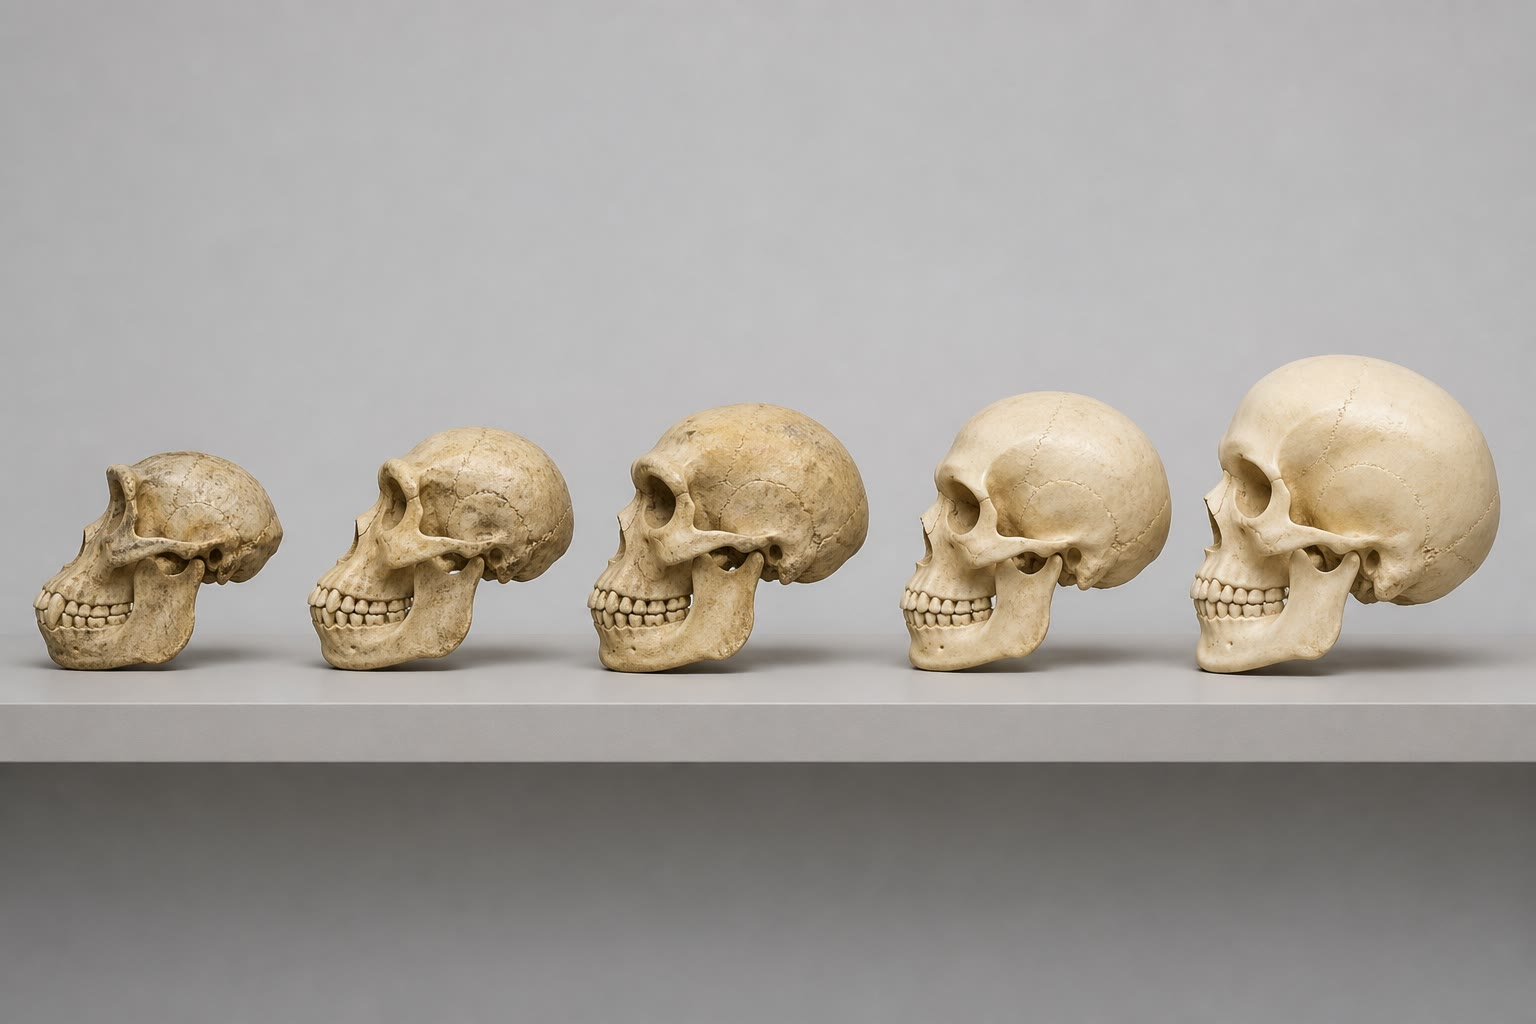
\includegraphics[width=0.66\linewidth]{images/book2/ai/g12-human-skulls.jpg}

{\small Crânios da linhagem vistos de lado, de um australopiteco a um
ser humano moderno: a caixa craniana incha, a face recua sob ela, a
arcada supraciliar some e aparece um queixo.}
\end{omfigure}

\begin{example}[Ler um crânio]\label{ex:g12:human-evolution:skull}
Um crânio fóssil com a abertura medular embaixo, uma caixa craniana de
\qty{450}{cm^3}, mandíbulas grandes e face projetada é um
australopiteco: ereto, de cérebro pequeno. Um com \qty{900}{cm^3},
arcada supraciliar pesada, testa fugidia e sem queixo é \emph{Homo
erectus}. Um com \qty{1400}{cm^3}, testa alta, face pequena encaixada
sob a caixa craniana e queixo é um ser humano moderno. A ordem desses
caracteres na árvore é a ordem em que eles aparecem nas rochas.
\end{example}

\section{Um arbusto, não uma escada}

\begin{proposition}[Várias espécies ao mesmo tempo]\label{prop:g12:human-evolution:bush}
A \omterm{def:g12:human-evolution:lineage}{linhagem humana} não é uma linha única de ancestrais e descendentes, e
sim um arbusto de \omterm{def:g10:biodiversity-scales:species}{espécies}, várias das quais viveram ao mesmo tempo:
dois ou três tipos de australopiteco há dois milhões de anos ao lado
dos primeiros \emph{Homo}; o \emph{Homo erectus} espalhado por três
continentes enquanto outras \omterm{def:g10:biodiversity-scales:species}{espécies} surgiam na África; e ainda há
cinquenta mil anos os seres humanos modernos dividiam a Terra com os
neandertais na Europa, outra \omterm{def:g12:selection-drift-speciation:population}{população} na Ásia e uma \omterm{def:g10:biodiversity-scales:species}{espécie} de corpo
pequeno numa ilha. A maioria dos ramos do arbusto terminou em extinção;
o nosso é o que ficou.
\end{proposition}
\begin{proof}[Evidence]
Fósseis de \omterm{def:g10:biodiversity-scales:species}{espécies} distintas são encontrados em camadas da mesma idade
nos mesmos sítios. Restos de neandertais e de seres humanos modernos se
sobrepõem na Europa por vários milhares de anos. O \omterm{def:g10:universal-dna:information}{DNA} dos neandertais
e o da \omterm{def:g12:selection-drift-speciation:population}{população} asiática, recuperado dos ossos deles, é distinto do
nosso --- e está presente em nós: as pessoas de fora da África carregam
cerca de 2\% de \omterm{def:g10:universal-dna:information}{DNA} neandertal, e algumas populações do Pacífico vários
por cento do da \omterm{def:g12:selection-drift-speciation:population}{população} asiática, o traço dos cruzamentos quando as
\omterm{def:g10:biodiversity-scales:species}{espécies} se encontraram. Os ramos se tocaram antes de terminar.
\end{proof}

\begin{omfigure}
\begin{tikzpicture}[font=\small]
  \tikzset{bar/.style={line width=6pt, line cap=butt}}
  % time axis: 0 at right, 4 Ma at left; 3 cm per Ma
  \draw[->, thick] (0,-0.4) -- (12.6,-0.4);
  \foreach \t/\l in {0/{4}, 3/{3}, 6/{2}, 9/{1}, 12/{0}} { \draw (\t,-0.3) -- (\t,-0.5); \node[anchor=north, font=\scriptsize] at (\t,-0.55) {\l}; }
  \node[anchor=north, font=\scriptsize] at (6.3,-0.95) {milhões de anos atrás};
  % species bars: (start, end) in Ma -> x = (4 - Ma)*3
  \draw[bar, omDef!60] (0.3,0.4) -- (3.3,0.4); \node[anchor=west, font=\scriptsize] at (3.4,0.4) {\emph{Australopithecus afarensis}};
  \draw[bar, omDef!60] (2.1,1.0) -- (5.7,1.0); \node[anchor=west, font=\scriptsize] at (5.8,1.0) {\emph{A. africanus}};
  \draw[bar, omDef!40] (3.9,1.6) -- (8.4,1.6); \node[anchor=west, font=\scriptsize] at (8.5,1.6) {\emph{Paranthropus}};
  \draw[bar, omProp!60] (4.8,2.2) -- (7.8,2.2); \node[anchor=west, font=\scriptsize] at (7.9,2.2) {\emph{Homo habilis}};
  \draw[bar, omProp!60] (6.3,2.8) -- (11.7,2.8); \node[anchor=west, font=\scriptsize] at (11.8,2.8) {\emph{H. erectus}};
  \draw[bar, omThm!50] (9.9,3.4) -- (11.4,3.4); \node[anchor=east, font=\scriptsize] at (9.8,3.4) {\emph{H. heidelbergensis}};
  \draw[bar, omThm!50] (10.8,4.0) -- (11.88,4.0); \node[anchor=east, font=\scriptsize] at (10.7,4.0) {neandertais};
  \draw[bar, omMeth!70] (11.1,4.6) -- (12.0,4.6); \node[anchor=east, font=\scriptsize] at (11.0,4.6) {\emph{H. sapiens}};
\end{tikzpicture}

{\small Algumas \omterm{def:g10:biodiversity-scales:species}{espécies} da \omterm{def:g12:human-evolution:lineage}{linhagem humana} e os períodos em que os
fósseis delas são encontrados. Em quase toda data, várias \omterm{def:g10:biodiversity-scales:species}{espécies}
coexistiram; a linhagem é um arbusto com um galhinho sobrevivente.}
\end{omfigure}

\begin{proposition}[Os seres humanos modernos]\label{prop:g12:human-evolution:sapiens}
O \emph{Homo sapiens} apareceu na África há cerca de 300\,000 anos,
reconhecível pelo crânio alto e arredondado, pela face pequena e pelo
queixo. Grupos pequenos saíram da África uns 60\,000 anos atrás e, em
50\,000 anos, tinham chegado a todos os continentes menos a Antártida,
encontrando e absorvendo em parte as populações mais antigas que
acharam. Todos os seres humanos vivos descendem daquela \omterm{def:g12:selection-drift-speciation:population}{população}
africana: a \omterm{def:g10:biodiversity-scales:biodiversity}{diversidade genética} da \omterm{def:g10:biodiversity-scales:species}{espécie} inteira é menor que a dos
chimpanzés de uma só região africana, e ela é maior na África,
diminuindo com a distância a partir dela ao longo das rotas de
dispersão --- a assinatura de grupos fundadores sucessivos.
\end{proposition}
\admitted

\begin{omfigure}
\begin{tikzpicture}
\begin{axis}[
  ybar, bar width=14pt,
  width=0.84\linewidth, height=5.2cm,
  axis x line=bottom, axis y line=left,
  ymin=0, ymax=6, ylabel={\% do genoma},
  ylabel style={font=\small},
  symbolic x coords={África subsaariana, Europa, Ásia Oriental, Melanésia},
  xtick=data, tick label style={font=\small},
  enlarge x limits=0.2, ytick={0,2,4,6},
  legend style={at={(0.03,0.95)}, anchor=north west, font=\small, draw=none},
]
\addplot[fill=omThm!50, draw=omThm] coordinates {(África subsaariana,0.1) (Europa,1.8) (Ásia Oriental,2.2) (Melanésia,2.0)};
\addplot[fill=omDef!50, draw=omDef] coordinates {(África subsaariana,0) (Europa,0) (Ásia Oriental,0.2) (Melanésia,3.5)};
\legend{DNA neandertal, DNA da população asiática}
\end{axis}
\end{tikzpicture}

{\small Parcela do genoma herdada de duas populações extintas, por
região (arredondada). As populações que saíram da África encontraram os
neandertais e se cruzaram com eles; as que chegaram ao Pacífico
ocidental encontraram também a \omterm{def:g12:selection-drift-speciation:population}{população} asiática. Os ramos do arbusto
trocaram \omterm{def:g10:universal-dna:gene}{genes} antes que todos menos um terminassem.}
\end{omfigure}

\section{O que nos fez}

\begin{proposition}[Os genes e, depois, a cultura]\label{prop:g12:human-evolution:culture}
Os caracteres da linhagem surgiram como os capítulos anteriores
descrevem: mutações, incluindo mudanças na regulação dos \omterm{prop:g12:diversification-of-life:development}{genes do
desenvolvimento} (um crescimento mais longo do cérebro, uma face mais
curta), separadas pela seleção nos ambientes das savanas africanas e
pela deriva em populações pequenas. Mas a linhagem acrescentou um
segundo modo de herança --- o comportamento transmitido do
\cref{ch:g12:diversification-of-life}, elevado a uma escala que nenhuma
outra \omterm{def:g10:biodiversity-scales:species}{espécie} alcançou: ferramentas, fogo, linguagem, cooperação,
ensino. A cultura se acumula dentro de uma vida e passa a todos os que
a aprendem, não só aos descendentes; nos últimos cem mil anos as
mudanças que mais importaram aos seres humanos foram culturais, e o
ambiente em que a \omterm{def:g10:biodiversity-scales:species}{espécie} evolui é, em boa parte, um ambiente que ela fez.
\end{proposition}
\admitted

\begin{method}[Situar um fóssil]\label{met:g12:human-evolution:placing}
\begin{enumerate}
  \item Date a camada (decaimento radioativo de minerais vulcânicos, ou
        a idade conhecida dos estratos).
  \item Leia o andar: posição da abertura medular, forma da bacia e do
        fêmur, o pé.
  \item Meça a caixa craniana; observe a face, a arcada supraciliar, o
        queixo, os dentes.
  \item Liste os estados derivados presentes e ausentes, e situe o
        fóssil na árvore pelas regras do
        \cref{ch:g12:phylogenetic-trees}: como um ramo lateral perto do
        nó em que a combinação de caracteres dele se encaixa, e não
        como ``o ancestral''.
  \item Onde o osso está bem conservado o bastante, leia o \omterm{def:g10:universal-dna:information}{DNA} e o
        compare com as populações vivas.
\end{enumerate}
\end{method}

\begin{remark}[Não há elo perdido]\label{rem:g12:human-evolution:link}
A expressão supõe uma corrente com uma lacuna; o registro é um arbusto
com muitos ramos, a maioria conhecida por alguns ossos, e o ``elo''
entre nós e o chimpanzé é um nó --- uma \omterm{def:g12:selection-drift-speciation:population}{população} extinta que não era
nem um nem outro --- e não uma criatura no meio do caminho. O que os
fósseis mostram, sim, na ordem em que as rochas os preservam, é cada
caráter derivado aparecendo na vez dele: os pés, depois os cérebros,
depois as ferramentas, depois o queixo --- e, nos últimos cinquenta mil
anos, as obras de uma \omterm{def:g10:biodiversity-scales:species}{espécie} cuja evolução hoje é, em boa parte, obra dela mesma.
\end{remark}

\section{Exercícios}

\begin{exercise}[$\star$]\label{exo:g12:human-evolution:1}
Qual \omterm{def:g10:biodiversity-scales:species}{espécie} viva é a parente mais próxima do ser humano, e há quanto
tempo as duas linhagens se separaram?
\end{exercise}

\begin{exercise}[$\star$]\label{exo:g12:human-evolution:2}
Liste quatro sinais esqueléticos do andar ereto.
\end{exercise}

\begin{exercise}[$\star$]\label{exo:g12:human-evolution:3}
A partir da figura do volume do cérebro, dê o volume de um
australopiteco, do \emph{Homo erectus} inicial e de um ser humano moderno.
\end{exercise}

\begin{exercise}[$\star$]\label{exo:g12:human-evolution:4}
Por que a \omterm{def:g12:human-evolution:lineage}{linhagem humana} é descrita como um arbusto, e não como uma escada?
\end{exercise}

\begin{exercise}[$\star$]\label{exo:g12:human-evolution:5}
Onde e quando o \emph{Homo sapiens} apareceu, e o que a distribuição da
\omterm{def:g10:biodiversity-scales:biodiversity}{diversidade genética} humana mostra?
\end{exercise}

\begin{exercise}[$\star\star$]\label{exo:g12:human-evolution:6}
O \omterm{def:g11:cell-cycle-mitosis:chromosome}{cromossomo} 2 humano corresponde a dois \omterm{def:g10:universal-dna:information}{cromossomos} de chimpanzé
unidos ponta a ponta. Explique como isso dá conta dos números
diferentes de \omterm{def:g10:universal-dna:information}{cromossomos}, e por que é uma evidência de parentesco, e
não contra ele.
\end{exercise}

\begin{exercise}[$\star\star$]\label{exo:g12:human-evolution:7}
O que veio primeiro na linhagem, o andar ereto ou um cérebro grande?
Por quanto tempo? Cite as evidências.
\end{exercise}

\begin{exercise}[$\star\star$]\label{exo:g12:human-evolution:8}
A partir da figura da linha do tempo, quais \omterm{def:g10:biodiversity-scales:species}{espécies} coexistiram há
dois milhões de anos? E há 100\,000 anos?
\end{exercise}

\begin{exercise}[$\star\star$]\label{exo:g12:human-evolution:9}
Uma pessoa de ascendência europeia carrega 2\% de \omterm{def:g10:universal-dna:information}{DNA} neandertal.
Explique que evento isso registra, e por que os africanos subsaarianos
quase não carregam nenhum.
\end{exercise}

\begin{exercise}[$\star\star$]\label{exo:g12:human-evolution:10}
Aplique o \cref{met:g12:human-evolution:placing} a um crânio com a
abertura medular adiantada, \qty{500}{cm^3}, mandíbulas grandes,
encontrado numa camada de 2.8 milhões de anos.
\end{exercise}

\begin{exercise}[$\star\star$]\label{exo:g12:human-evolution:11}
Explique por que ``os seres humanos descendem dos primatas antropoides''
se enuncia corretamente como ``os seres humanos são primatas
antropoides'', usando o vocabulário dos \omterm{prop:g12:phylogenetic-trees:rules}{clados}.
\end{exercise}

\begin{exercise}[$\star\star\star$]\label{exo:g12:human-evolution:12}
Os neandertais tinham cérebros ligeiramente maiores que os nossos e
faziam ferramentas sofisticadas, e mesmo assim desapareceram em alguns
milhares de anos depois da nossa chegada à Europa. Proponha duas
hipóteses compatíveis com o capítulo e diga que evidência as distinguiria.
\end{exercise}

\begin{exercise}[$\star\star\star$]\label{exo:g12:human-evolution:13}
A \omterm{def:g10:biodiversity-scales:biodiversity}{diversidade genética} humana diminui com a distância a partir da
África ao longo das rotas de dispersão. Explique isso com o efeito
fundador do \cref{ch:g12:selection-drift-speciation}, e diga o que ele
implica sobre como a dispersão aconteceu.
\end{exercise}

\begin{exercise}[$\star\star\star$]\label{exo:g12:human-evolution:14}
A persistência da lactase, a pele clara em latitudes altas e a
resistência à malária são caracteres humanos que evoluíram nos últimos
dez mil anos. Explique como uma mudança cultural (a pecuária leiteira,
a migração, a agricultura) consegue criar a seleção que muda os \omterm{def:g10:universal-dna:gene}{genes}.
\end{exercise}

\begin{exercise}[$\star\star\star$]\label{exo:g12:human-evolution:15}
``A evolução parou para os seres humanos, já que a medicina e a cultura
nos protegem da seleção.'' Discuta num parágrafo, com a deriva, os três
caracteres do exercício anterior e o sentido da seleção.
\end{exercise}

\section{Problema: os caminhantes na cinza}

\begin{problem}[{Problema de fim de semana --- dois rastros de pegadas
lidos quanto ao andar, à altura e à velocidade; uma fileira de crânios
medida; e o DNA de uma estudante viva rastreado até três populações}]
\label{pb:g12:human-evolution:1}
Dois rastros de pegadas, de 3.6 milhões de anos, correm paralelos por
\qty{27}{m}. Rastro A: comprimento da pegada \qty{21.5}{cm}, passada
(de uma marca à seguinte do mesmo pé) \qty{0.95}{m}. Rastro B:
comprimento \qty{18.5}{cm}, passada \qty{0.80}{m}. Nos seres humanos
modernos o pé é cerca de 15\% da altura em pé, e uma passada de andar
de cerca de 0.8 vez a altura corresponde a um andar lento.

\medskip
\noindent\textbf{Parte I --- As pegadas.}
\begin{enumerate}
  \item Estime a altura do caminhante A e a do caminhante B.
  \item Compare cada passada com 0.8 vez a altura. Eles estavam
        andando ou correndo?
  \item As marcas mostram um calcanhar fundo, um arco e um dedão
        paralelo aos outros. O que cada característica mostra sobre o
        pé e sobre o andar?
  \item Um chimpanzé que anda ereto deixa marcas com a sola plana e o
        dedão divergente, e não consegue manter isso por muito tempo.
        Quais caracteres da \cref{prop:g12:human-evolution:bipedalism}
        os rastros estabelecem para quem os fez, e quais eles deixam
        desconhecidos?
  \item Os fósseis mais próximos da mesma idade têm cérebros de
        \qty{400}{cm^3}. O que a combinação --- estes pés, aquele
        cérebro --- resolve sobre a ordem dos caracteres da linhagem?
\end{enumerate}

\medskip
\noindent\textbf{Parte II --- Os crânios.}
Cinco crânios, com volume da caixa craniana, idade e características:
1: \qty{450}{cm^3}, 3.0 milhões de anos, face projetada, sem queixo.
2: \qty{650}{cm^3}, 1.9 milhão de anos, face menor.
3: \qty{950}{cm^3}, 1.0 milhão de anos, arcada pesada, sem queixo.
4: \qty{1450}{cm^3}, 60\,000 anos, arcada pesada, sem queixo, crânio
longo e baixo.
5: \qty{1350}{cm^3}, 30\,000 anos, testa alta, queixo.
\begin{enumerate}[resume]
  \item Atribua cada crânio a um grupo da figura da linha do tempo.
  \item Trace, ou descreva, o volume do cérebro contra a idade dos
        cinco. Em que intervalo o volume cresce mais rápido?
  \item O crânio 4 é maior que o crânio 5. O volume do cérebro sozinho
        identifica um ser humano moderno? Quais caracteres identificam?
  \item Os crânios 4 e 5 se sobrepõem no tempo. O que o capítulo diz
        sobre a relação entre as duas populações deles, e que evidência
        sustenta isso?
  \item O crânio 1 e as pegadas da Parte I poderiam pertencer à mesma
        \omterm{def:g10:biodiversity-scales:species}{espécie}. Explique por que essa \omterm{def:g10:biodiversity-scales:species}{espécie} é um \emph{parente}
        parecido com um ancestral, e não um ancestral demonstrado, na
        linguagem do \cref{ch:g12:phylogenetic-trees}.
\end{enumerate}

\medskip
\noindent\textbf{Parte III --- O genoma da estudante.}
Uma estudante de ascendência europeia e melanésia tem o genoma dela
comparado com os dos neandertais e com o da \omterm{def:g12:selection-drift-speciation:population}{população} asiática extinta:
1.6\% bate com o genoma neandertal, 1.8\% com o asiático.
\begin{enumerate}[resume]
  \item Explique o que uma correspondência de 1.6\% significa e que
        evento ela registra.
  \item Compare os números dela com o gráfico. Quais das populações
        ancestrais dela contribuíram com cada parcela?
  \item Se os cruzamentos ocorreram há 50\,000 anos e uma geração é de
        25 anos, quantas gerações a separam do evento? Por que a
        parcela não foi diluída até sumir?
  \item Duas linhagens contribuíram com \omterm{def:g10:universal-dna:gene}{genes} para a dela embora sejam
        chamadas de \omterm{def:g10:biodiversity-scales:species}{espécies}. O que isso diz sobre a fronteira de
        \omterm{def:g10:biodiversity-scales:species}{espécie} do \cref{ch:g12:selection-drift-speciation} naquela época?
  \item O \omterm{def:g10:universal-dna:information}{DNA} mitocondrial dela é do tipo humano moderno, como o de
        toda pessoa viva. O que isso mostra sobre a direção ou sobre o
        destino dos cruzamentos?
\end{enumerate}

\medskip
\noindent\textbf{Parte IV --- O relógio e o arbusto.}
\begin{enumerate}[resume]
  \item O \omterm{def:g10:universal-dna:information}{DNA} humano e o do chimpanzé diferem em 1.2\%; o relógio dos
        primatas do \cref{ch:g12:phylogenetic-trees} corre a 0.27\% por
        milhão de anos. Date o ancestral comum.
  \item Os fósseis mais antigos conhecidos da \omterm{def:g12:human-evolution:lineage}{linhagem humana} têm de 6
        a 7 milhões de anos. Isso é coerente com a sua data?
  \item Liste as \omterm{def:g10:biodiversity-scales:species}{espécies} da linha do tempo que estavam vivas há um
        milhão de anos, e diga quantas delas têm descendentes vivos.
  \item Explique por que os últimos cem mil anos da linhagem são
        descritos melhor pela mudança cultural que pelos caracteres
        deste capítulo.
  \item Enuncie o resultado: a altura e o andar do caminhante A, a
        ordem em que os pés, o cérebro e o queixo apareceram, e o
        número de populações extintas cujos \omterm{def:g10:universal-dna:gene}{genes} a estudante carrega.
\end{enumerate}
\end{problem}
